% !TeX spellcheck = es_ES
% !TeX encoding = UTF-8
\documentclass[10pt,handout]{beamer}

% Language
\usepackage[spanish]{babel}
\usepackage[utf8]{inputenc}
\usepackage[T1]{fontenc}

\setbeamersize{text margin left=5mm, text margin right=5mm}
\usetheme{metropolis}

\usepackage{tikz}

% --- Essentials ---
\usepackage{appendixnumberbeamer}
\usepackage{booktabs}
\usepackage[scale=2]{ccicons}
\usepackage{pgfplots}
\usepgfplotslibrary{dateplot}
\usepackage{xspace}
\usepackage{graphicx}\graphicspath{{figs/}{/home/jadeleon/Documents/doctorado/protocolo_candidatura/gfx/background}{/home/jadeleon/Documents/doctorado/protocolo_candidatura/gfx/chaos_meets_channels/}{/home/jadeleon/Documents/chaos_meets_channels/posters/pix}}
\usepackage{physics}
\usepackage{amsmath}
%\usepackage{siunitx}

% --- Bibliography setup ---
\usepackage[%
    style=verbose,
    backend=bibtex,
    giveninits=true,      % Use initials for first names
    isbn=false, url=false, doi=false, eprint=false,
    maxcitenames=1,
    mincitenames=1
]{biblatex}

% Custom format: Author, Journal, vol, page, (year)
\DeclareFieldFormat[article]{journaltitle}{#1}
\DeclareFieldFormat[article]{volume}{\textbf{#1}} % Bold volume number
\DeclareFieldFormat[article]{pages}{#1} % Remove "p." for cleaner look

% Redefine the short citation format for verbose style
\renewbibmacro*{cite:short}{%
  \color{gray}\tiny
  \printtext[brackets]{%
    \printfield{journaltitle}%
    \setunit*{\space}%
    \printfield{volume}%
    \setunit*{\space}%
    \printfield{pages}%
    \setunit*{\space}%
    \printtext[parens]{\printfield{year}}%
  }
}

% Also modify the full citation format for consistency
\renewbibmacro*{cite:full}{%
  \color{gray}\tiny
  \printtext[brackets]{%
    \printfield{journaltitle}%
    \setunit*{\space}%
    \printfield{volume}%
    \setunit*{\space}%
    \printfield{pages}%
    \setunit*{\space}%
    \printtext[parens]{\printfield{year}}%
  }
}

%\addbibresource{references.bib}
\addbibresource{/home/jadeleon/Documents/doctorado/protocolo_candidatura/references.bib}

% --- Single, clean inline citation command ---
\newcommand{\scite}[1]{\textcolor{gray}{\scriptsize(\citeauthor{#1}, \citeyear{#1})}}

% --- Colors and theme styling ---
\definecolor{deepblue}{RGB}{46,78,126}
\definecolor{lightblue}{RGB}{200,220,255}
\setbeamercolor{palette primary}{bg=deepblue, fg=white}
\setbeamercolor{palette secondary}{bg=deepblue, fg=white}
\setbeamercolor{palette tertiary}{bg=deepblue, fg=white}
\setbeamercolor{structure}{fg=deepblue}

% --- Metadata ---
\title{Pureza de Choi-Jamiolkowski como indicador de caos cuántico de muchos cuerpos}
%\subtitle{Brief Subtitle Explaining Domain}
\date{\today}
\author{\textbf{Jose Alfredo de Leon}\inst{1} \and 
Miguel Gonzalez\inst{2} \and
Carlos Diaz-Mejia\inst{2}}
\institute{
\inst{1}Instituto de Física, UNAM
\and 
\inst{2}Instituto de Ciencias Nucleares, UNAM
}
%\titlegraphic{\hfill\includegraphics[height=1cm]{logo.pdf}}

% ------------
\newcommand{\choip}{\ev{\Tr[\mathcal{D}^2(t)]}_{\mathrm{Haar},t}}
\newcommand{\statep}{\overline{\mathcal{P}}}


\begin{document}

\maketitle

\begin{frame}{¿Cómo diagnosticar caos cuántico de muchos cuerpos?}
\begin{itemize}
\item Propiedades estadísticas del Hamiltoniano $\rightarrow$ matriz aleatoria

\begin{center}
\includegraphics[height=0.5\textheight]{many-body.pdf}
\end{center}

\item Desafío: Acceso limitado a propiedades completas del sistema
\end{itemize}

{\tiny \color{gray} [PRA \textbf{93} 063632 (2016)]}
\end{frame}

\begin{frame}{Caos cuántico monitoreando sistemas reducidos}
\begin{columns}[T]
\column{0.49\textwidth}
Monitoreo de la pureza
\begin{center}
\includegraphics[width=\textwidth]{fig1_mirkin.png}
\end{center}
\vspace*{-2mm}
\cite{mirkin_2021_quantum}

\column{0.49\textwidth}
Reavivamientos en el factor de decoherencia
\begin{center}
\includegraphics[width=\textwidth]{fig1_mirkin2021b.png}
\end{center}
\cite{mirkin_2021_sensing}
\end{columns}
\end{frame}

% --- Opening, motivation ----
\begin{frame}
\vspace*{-5mm}
\begin{center}
\includegraphics[height=\textheight]{idea.pdf}
\end{center}

%\begin{center}
\begin{tikzpicture}[overlay, remember picture, shift={(current page.center)}]
% Caja con fondo degradado
\node[fill=orange!30, 
      draw=orange!80!black,
      thick,
      rounded corners=10pt,
      inner sep=5pt,
      minimum width=0.6\linewidth,
      align=center] at (0,-3.8) {
    \textcolor{orange!80!black}{¿Señales de caos en el canal cuántico $\mathcal{E}$?}\\
    \textcolor{black}{\textbf{Pureza de Choi}}
};

\end{tikzpicture}
%\end{center}
\end{frame}

% --- Quantum channels ----
\begin{frame}{Canales cuánticos}
Describen ruido cuántico, mediciones generalizadas y \alert{dinámica de 
sistemas cuánticos abiertos}. 

\begin{columns}[t,onlytextwidth]
\column{0.47\textwidth}
\metroset{block=fill}
\begin{alertblock}{Representación sistema-entorno}
Para todo $\mathcal{E}$, existe $\{U, \ket{\psi}\}$:
\[
\mathcal{E}(\rho) 
=
\Tr_\mathrm{E}
\qty(
U 
\rho \otimes \dyad{\psi}
U^\dagger
).
\]
%
\begin{center}
\begin{tikzpicture}[font=\large, thick, >=stealth, transform shape, scale=0.8]

% --- Bloque U ---
\draw[rounded corners=6pt, thick] (0,0) rectangle (2,3.5);
\node at (1,2) {$U$};

% --- Bloque E (dentro de U, sombreado) ---
\draw[dashed, rounded corners=6pt, thick] (-0.1,0.1) rectangle (2.1,1.6);
\node at (1,0.85) {$\mathcal{E}$};

% --- Líneas de entrada y salida ---
\draw[-] (-1,0.85) -- (0,0.85);
\draw[-] (-1,2.5) -- (0,2.5);
\draw[-] (2,0.85) -- (3.1,0.85);

% --- Etiquetas de las líneas ---
\node[left] at (-1,2.5) {$\dyad{\psi}$};
\node[left] at (-1,0.85) {$\rho$};
\node[right] at (3.1,0.85)
%    {$\mathrm{Tr}_\mathrm{E}(U \rho \otimes \dyad{\psi} U^{\dagger})$};
     {$\mathcal{E}(\rho)$};
\end{tikzpicture}
\end{center}
\end{alertblock}

\column{0.47\textwidth}
\metroset{block=fill}
\begin{alertblock}{Representación de Choi}
A $\mathcal E$ le corresponde un único \alert{estado}
\[\begin{aligned}
\mathcal{D} &= 
\qty(\mathcal{E} \otimes I )
\qty[\dyad{\Phi}],\\
\ket{\Phi} &= 
\frac{1}{\sqrt{d}}
\sum_i \ket{i}\otimes \ket{i}.
\end{aligned}\]

\begin{itemize}
\item $\mathcal{D} \in \mathcal{B}(\mathcal H \otimes \mathcal H)$
\item $\frac{1}{d^2} \leq \Tr(\mathcal{D}^2) \leq 1$
\end{itemize}
\end{alertblock}
\end{columns}

\end{frame}
% --- Quantum chaos ----
\begin{frame}[t]{Caos cuántico}
\begin{columns}[onlytextwidth]
\column{0.35\textwidth}

\metroset{block=fill}
\begin{alertblock}{\color{black} Caos cuántico = RMT}
\begin{center}
\includegraphics[width=0.95\textwidth]{random_goe.pdf}
\end{center}
\end{alertblock}

\column{0.63\textwidth}
\vspace*{-2mm}
\metroset{block=fill}
\begin{alertblock}{Eigenvalores correlacionados}
\begin{itemize}
\item Repulsión de niveles
\hspace*{27mm}
\includegraphics[height=25mm,page=2]{spacings.pdf}
\vspace*{-3mm}
\item $SFF(t) = \sum_{i,j} e^{-i (E_i - E_j) t}$
\begin{center}
\includegraphics[height=24mm]{sff.png}
\end{center}
\end{itemize}
\vspace*{-2mm}
\end{alertblock}

\begin{exampleblock}{Eigenvectores deslocalizados}
\vspace*{-2mm}
\begin{center}
$\ket{E_i} \approx \ket{\psi_{\mathrm{random}}}$
\end{center}
\vspace*{-2mm}
\end{exampleblock}
\end{columns}

%\vspace*{-5mm}
%\cite{bohigas_1984_characterization}
%\cite{berry_1997_level}

\begin{tikzpicture}[overlay, remember picture, shift={(current page.center)}]
\node[xshift=4mm, yshift=20mm] at (current page.center) 
{\tiny$
\begin{aligned}
\tilde r_n &= \frac{E_{n+1} - E_n}{E_{n} - E_{n-1}},
r_n = \min\left(\tilde r_n, \frac{1}{\tilde r_n}\right)
%r_n = \min\qty( \frac{E_{n+1} - E_n}{E_{n} - E_{n-1}}, \frac{E_{n+1} - E_n}{E_{n} - E_{n-1}})
\end{aligned}
$};
%
\node[xshift=2mm, yshift=12mm] at (current page.center) 
{\tiny $
\begin{aligned}
\ev{r}_{\mathrm{GOE}} &\approx 0.536 \\
\ev{r}_{\mathrm{Poisson}} &\approx 0.386
\end{aligned}
$};
%
\node[xshift=7mm, yshift=4mm] at (current page.center) 
{\tiny \color{gray} [PRL \textbf{110} 084101 (2013)]};
\end{tikzpicture}
\end{frame}

\begin{frame}{Pureza de Choi como indicador de caos}
Dado un Hamiltoniano $H$,
\begin{equation*}
\mathcal{E}_t(\rho) 
=
\Tr_\mathrm{E}
\qty(
e^{-i H t}
\rho \otimes \dyad{\psi}
e^{i H t}
),\quad 
\ket{\psi} = \bigotimes_i \ket{\phi_i}.
\end{equation*}

\begin{columns}[T,onlytextwidth]
\column{0.49\textwidth}
\textbf{¿Cómo se ve el canal cuántico $\mathcal E_t$?}

\vspace*{2mm}

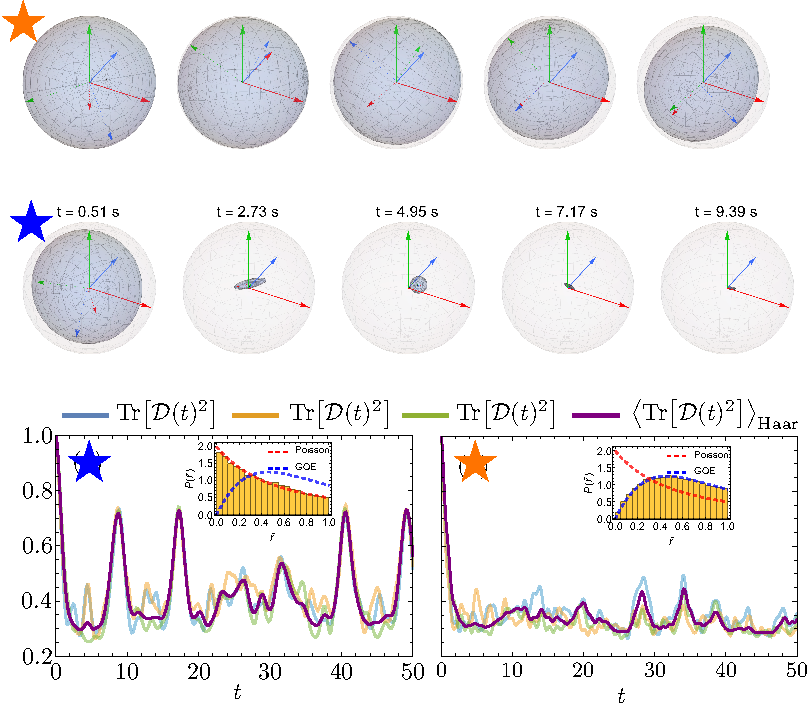
\includegraphics[width=\linewidth]{channel.pdf}

\column{0.49\textwidth}
\metroset{block=fill}
\begin{alertblock}{Promedio de Haar de $\Tr[\mathcal{D}(t)^2]$}
\begin{itemize}
\item El caos está en $H$
\item Sin embargo, $\mathcal E$ depende de $\ket{\psi}$
\item Removemos \alert{analíticamente} la dependencia en $\ket{\psi}$: 
\vspace*{-4mm}
\begin{equation*}
\scalebox{0.45}{$
\underset{\ket{\phi_i} \sim \mu_{\mathrm{Haar}} }
{\mathbb{E}\qty[\Tr \mathcal{D}^2(t)]} 
= 
\frac{1}{12^{L-1}} \sum_{\vec{k} \in 
\{0,1,2,3\}^{L-1}} 3^{\frac{1}{2}\qty(L - 1 - w\qty(\vec{k}))} 
\Tr \qty[ \Tr_S^2 \qty(U(t) \sigma_{0,\vec{k}}\, U^\dagger(t)) ]
$}
\end{equation*}

\item \alert{Vamos a usar el siguiente número como indicador de caos:}
\begin{equation*}
\scalebox{0.9}{$
\ev{\Tr \mathcal{D}^2(t)}_{\mathrm{Haar}, t} = 
\int_0^T
\underset{\ket{\phi_i} \sim \mu_{\mathrm{Haar}} }
{\mathbb{E}\qty[\Tr \mathcal{D}^2(t)]} 
\dd{t}
$}
\end{equation*}
\end{itemize}
\end{alertblock}
\end{columns}

\end{frame}

% --- Resultados ---
\begin{frame}{Modelo de Ising con campos transverso y longitudinal}
\[
H = \sum_{i=1}^L \left( h_x \sigma_i^x + h_z \sigma_i^z \right) 
- J \sum_{i=1}^{L-1} \sigma_i^z \sigma_{i+1}^z,
\]
\begin{center}
\begin{tikzpicture}
%------------------------------------- Panel a -------------------------------
\begin{scope}[shift={(0,0)}, scale=0.8, transform shape]
% Mean level spacing ratio
\node (listdensityplotr) at (0,0) {\includegraphics[width=0.325\textwidth]{mean_level_spacing_ratio_ising_L_16_hx_1_even_parity.pdf}};
\node[rotate=90] () at (listdensityplotr.west) [] {$J/h_x$};
\node (barlegend) at (listdensityplotr.north) [anchor=south, inner sep=-10pt]  {\includegraphics[width=0.27\textwidth]{mean_level_spacing_ratio_ising_bar_legend.pdf}};
\node (labelr) at (barlegend.north) [anchor=south, inner sep=10pt] {$\ev{\tilde r_n}$};
%\node () at ([xshift=-45pt]labelr.west) {(a)};
\node () at (listdensityplotr.south) [anchor=north, inner sep=-5pt] {$h_z/h_x$};
% Texto L=7 dentro de la figura, esquina inferior derecha
\node[anchor=south east, font=\normalsize, inner sep=20pt] at (listdensityplotr.south east) {\color{white} $L=16$};

% Averaged purity
\node (chaometer) at (4.4,0) {\includegraphics[height=0.345\textwidth]{chaometer_purity_ising_L_7_hx_1.pdf}};
\node (legendChaometer) at (chaometer.north) [anchor=south, inner sep=-10pt]  {\includegraphics[width=0.27\textwidth]{chaometer_purity_ising_bar_legend.pdf}};
\node (labelChaometer) at (legendChaometer.north) [anchor=south, inner sep=10pt] {$\overline{\mathcal{P}}$};
\node () at (chaometer.south) [anchor=north, inner sep=-5pt] {$h_z/h_x$};
% Texto L=7 dentro de la figura, esquina inferior derecha
\node[anchor=south east, font=\normalsize, inner sep=20pt] at (chaometer.south east) {\color{white} $L=7$};

% Averaged Choi purity
\node (choi) at (8.95, -0.07) {\includegraphics[height=0.33\textwidth]{temporal_avg_haar_avg_choi_purity_ising_L_7_hx_1.pdf}};
\node (legendChoi) at (choi.north) [anchor=south, inner sep=-2pt]  {\includegraphics[width=0.27\textwidth]{temporal_avg_haar_avg_choi_purity_ising_bar_legend.pdf}};
\node (labelchoi) at (legendChoi.north) [anchor=south, inner sep=4pt] {$\ev{\Tr[\mathcal{D}(t)^2]}_{\mathrm{Haar}, t}$};
\node () at (choi.south) [anchor=north, inner sep=-5pt] {$h_z/h_x$};
% Texto L=7 dentro de la figura, esquina inferior derecha
\node[anchor=south east, font=\normalsize, inner sep=20pt] at (choi.south east) {\color{white} $L=7$};
\end{scope}

%%------------------------------------- Panel b -------------------------------
%\begin{scope}[shift={(0,-6)}]
%% Mean level spacing ratio 
%\node (listdensityplotr) at (0,0.05) {\includegraphics[width=0.325\textwidth]{mean_level_spacing_ratio_xxz_L_18_spinsUp_7_d_9_omega_0.pdf}};
%\node[rotate=90] () at ([xshift=-3pt,yshift=0pt]listdensityplotr.west) [] {$J_{xy}/J_z$};
%\node (barlegend) at (listdensityplotr.north) [anchor=south, inner sep=-7pt]  {\includegraphics[width=0.27\textwidth]{mean_level_spacing_ratio_ising_bar_legend.pdf}};
%\node () at ([xshift=-15pt,yshift=5pt]barlegend.west) {(b)};
%\node () at (listdensityplotr.south) [anchor=north, inner sep=-5pt] {$\varepsilon/J_z$};
%
%% Averaged purity
%\node (chaometer) at (4.47,0) {\includegraphics[height=0.333\textwidth]{chaometer_purity_xxz_open_L_7_d_3_Jz_1.00_omega_0.00.pdf}};
%\node (legendChaometer) at (chaometer.north) [anchor=south, inner sep=-2pt]  {\includegraphics[width=0.27\textwidth]{chaometer_purity_xxz_bar_legend.pdf}};
%\node () at (chaometer.south) [anchor=north, inner sep=-5pt] {$\varepsilon/J_z$};
%
%% Averaged Choi purity
%\node (choi) at (8.95, 0) {\includegraphics[height=0.333\textwidth]{temporal_avg_haar_avg_choi_purity_xxz_L_7_Jz_1_omega_0_d_3.pdf}};
%\node (legendChoi) at (choi.north) [anchor=south, inner sep=-2pt]  {\includegraphics[width=0.27\textwidth]{temporal_avg_haar_avg_choi_purity_xxz_bar_legend.pdf}};
%\node () at (choi.south) [anchor=north, inner sep=-5pt] {$\varepsilon/J_z$};
%\end{scope}
%
%\begin{scope}[anchor=north west, shift={(0,-8.9)}]
%\node[anchor=north west] (g) at (0, 0) {\includegraphics[width=0.65\textwidth]{heisenberg.pdf}};
%\node () at (g.south) [anchor=north, inner sep=-5pt] {$h$};
%\node(label1) at (1.6,-3.45) {$7$ $\uparrow$};
%\node () at ([xshift=0pt,yshift=7pt]g.north west) {(c)};
%\node(label2) at ([xshift=0pt,yshift=-5pt]label1.north) [anchor=south] {$13$ $\uparrow$};
%\node(label3) at ([xshift=0pt,yshift=-3pt]label2.north) [anchor=south, inner ysep=0pt] {$6$ $\uparrow$};
%\node(label4) at ([xshift=0pt,yshift=1pt]label3.north) [anchor=south, inner ysep=0pt] {$5$ $\uparrow$};
%\node(label5) at ([xshift=0pt,yshift=2pt]label4.north) [anchor=south, inner ysep=0pt] {$4$ $\uparrow$};
%\node() at ([xshift=-8pt,yshift=2pt]label5.north) [anchor=south, inner ysep=0pt] {$\ev{\tilde r}$};
%
%\node(labelgoe) at (4.92, -0.43) {$\ev{\tilde{r}}_\mathrm{GOE}$};
%\node() at ([xshift=12pt,yshift=0pt]labelgoe.east) [anchor=west, inner sep=0pt] {$\ev{\tilde{r}}_\mathrm{Poisson}$};
%\node(labelChoi) at ([xshift=-20pt,yshift=4pt]labelgoe.south) [anchor=north west] {\small $1 - \ev{\Tr[\mathcal{D}(t)^2]}_{\mathrm{Haar},t}$};
%\node(labelP) at ([xshift=-33.5pt,yshift=8pt]labelChoi.south) [anchor=north] {\small $1- \overline{\mathcal{P}}$};
%\end{scope}
\end{tikzpicture}
\end{center}

\begin{itemize}
\item ¡¡Cadenas mucho más pequeñas para $\statep$ y $\choip$!!
\item Para $J >1$ la resolución de $\choip$ se vuelve mejor que la de 
$\statep$ 
\end{itemize}
\end{frame}

\begin{frame}{Modelo de Heisenberg con campos aleatorios}

\[
H = \frac{1}{4}\sum_{i=1}^{L-1} \left(\sigma_i^x\sigma_{i+1}^x 
+ \sigma_i^y\sigma_{i+1}^y + \sigma_i^z\sigma_{i+1}^z\right) 
+ \frac{1}{2}\sum_{i=1}^L h_i \sigma_i^z,
\quad 
h_i \sim [-h,h]
\]
\begin{center}
\begin{tikzpicture}
\begin{scope}[anchor=north west, shift={(0,-8.9)}, scale=0.95, transform shape]
\node[anchor=north west] (g) at (0, 0) {\includegraphics[width=0.65\textwidth]{heisenberg.pdf}};
\node () at (g.south) [anchor=north, inner sep=-5pt] {$h$};
\node(label1) at (1.4,-3) {$7$ $\uparrow$};
\node(label2) at ([xshift=0pt,yshift=-5pt]label1.north) [anchor=south] {$13$ $\uparrow$};
\node(label3) at ([xshift=0pt,yshift=-3pt]label2.north) [anchor=south, inner ysep=0pt] {$6$ $\uparrow$};
\node(label4) at ([xshift=0pt,yshift=1pt]label3.north) [anchor=south, inner ysep=0pt] {$5$ $\uparrow$};
\node(label5) at ([xshift=0pt,yshift=2pt]label4.north) [anchor=south, inner ysep=0pt] {$4$ $\uparrow$};
\node() at ([xshift=-7pt,yshift=3pt]label5.north) [anchor=south, inner ysep=0pt] {$\ev{\tilde r}$};

\node(labelgoe) at (4.2, -0.43) {$\ev{\tilde{r}}_\mathrm{GOE}$};
\node() at ([xshift=7pt,yshift=0pt]labelgoe.east) [anchor=west, inner sep=0pt] {$\ev{\tilde{r}}_\mathrm{Poisson}$};
\node(labelChoi) at ([xshift=-18pt,yshift=4pt]labelgoe.south) [anchor=north west] {\small $1 - \ev{\Tr[\mathcal{D}(t)^2]}_{\mathrm{Haar},t}$};
\node(labelP) at ([xshift=-30pt,yshift=8pt]labelChoi.south) [anchor=north] {\small $1- \overline{\mathcal{P}}$};
\end{scope}
\end{tikzpicture}
\end{center}

\begin{itemize}
\item $\choip$ tiene una desviación estándar no visible al ojo
en la región de caos
\end{itemize}
\end{frame}

\begin{frame}{Modelo XXZ con defecto local}
\[
H = \frac{1}{4}\sum_{i=1}^{L-1} \left[ J_{xy} \left(\sigma_i^x\sigma_{i+1}^x 
+ \sigma_i^y\sigma_{i+1}^y \right) + J_z \sigma_i^z\sigma_{i+1}^z \right] 
+ \frac{1}{2}\varepsilon \sigma_d^z.
\]
\begin{center}
\begin{tikzpicture}
\begin{scope}[shift={(0,-6)}, scale=0.8, transform shape]
% Mean level spacing ratio 
\node (listdensityplotr) at (0,0.05) {\includegraphics[width=0.325\textwidth]{mean_level_spacing_ratio_xxz_L_18_spinsUp_7_d_9_omega_0.pdf}};
\node[rotate=90] () at ([xshift=-3pt,yshift=0pt]listdensityplotr.west) [] {$J_{xy}/J_z$};
\node (barlegend) at (listdensityplotr.north) [anchor=south, inner sep=-7pt]  {\includegraphics[width=0.27\textwidth]{mean_level_spacing_ratio_ising_bar_legend.pdf}};
%\node () at ([xshift=-15pt,yshift=5pt]barlegend.west) {(b)};
\node () at (listdensityplotr.south) [anchor=north, inner sep=-5pt] {$\varepsilon/J_z$};

% Averaged purity
\node (chaometer) at (4.47,0) {\includegraphics[height=0.333\textwidth]{chaometer_purity_xxz_open_L_7_d_3_Jz_1.00_omega_0.00.pdf}};
\node (legendChaometer) at (chaometer.north) [anchor=south, inner sep=-2pt]  {\includegraphics[width=0.27\textwidth]{chaometer_purity_xxz_bar_legend.pdf}};
\node () at (chaometer.south) [anchor=north, inner sep=-5pt] {$\varepsilon/J_z$};

% Averaged Choi purity
\node (choi) at (8.95, 0) {\includegraphics[height=0.333\textwidth]{temporal_avg_haar_avg_choi_purity_xxz_L_7_Jz_1_omega_0_d_3.pdf}};
\node (legendChoi) at (choi.north) [anchor=south, inner sep=-2pt]  {\includegraphics[width=0.27\textwidth]{temporal_avg_haar_avg_choi_purity_xxz_bar_legend.pdf}};
\node () at (choi.south) [anchor=north, inner sep=-5pt] {$\varepsilon/J_z$};
\end{scope}
\end{tikzpicture}
\end{center}

\begin{itemize}
\item Un sólo defecto es capaz de romper la integrabilidad~\cite{santos_2004_integrability}
\item $\statep$ y $\choip$ deben capturar correlaciones mezcladas de espacios
distintos.
\end{itemize}
\end{frame}

% --- Qué mira la pureza? ----
\begin{frame}{¿Qué captura la pureza de Choi?}
Para un canal cuántico arbitrario 
\[
\mathcal{E}(\rho) 
=
\Tr_\mathrm{E}
\qty(
U 
\rho \otimes \dyad{\psi}
U^\dagger
)
\]
la pureza de Choi puede escribirse:
\[
\Tr(\mathcal{D}^2) = 
\ev**{
\Tr_S\qty{
{\color{green} U^\dagger 
{\color{blue}\Lambda \qty[
{\color{red} U 
{\color{black} \left( \frac{I_2}{2} \otimes \dyad{\psi} \right)} 
U^\dagger}
]}
U}
}
}{\psi},
\]
\begin{itemize}
\item Evolución para adelante $\color{red} U$ 
\item Un proceso de ruido blanco sobre el sistema $\color{blue}\Lambda$
\item Evolución para atrás $\color{green}U^\dagger$
\end{itemize}
\pause
\alert{La pureza de Choi cuantifica la irreversibilidad de la evolución ante
una perturbación que destruye el entrelazamiento.}
\begin{tikzpicture}[overlay, remember picture, shift={(current page.center)}]
% Caja con fondo degradado
\node[fill=orange!30, 
      draw=orange!80!black,
      thick,
      rounded corners=10pt,
      inner sep=5pt,
      minimum width=0.35\linewidth,
      align=center] at (4, -1.5) {
    \textcolor{orange!80!black}{Echo de Loschmidt}\\
    \textcolor{black}{$\mel{\psi_0}{e^{i (H + V) t}e^{-i H t}}{\psi_0}$}
};
\end{tikzpicture}
\end{frame}

% --- Thank you slide ---
\begin{frame}[standout]
  \centering
  Muchas gracias\\
  \vspace{2cm}
  ¿Preguntas?\\
  \vspace{2cm}
  \small Jose Alfredo de Leon\\
  \texttt{deleongarrido.jose@gmail.com}\\
%  \vspace{0.5cm}
%  \tiny References available upon request
\end{frame}

% --- References slide ---
%\begin{frame}[allowframebreaks]{References}
%  \printbibliography[heading=none]
%\end{frame}

\end{document}